\documentclass[a4paper,12pt]{article}
\usepackage{caption}
\usepackage{float}
\usepackage{graphicx}
\usepackage{listings}
\usepackage{amsfonts}
\usepackage{amsmath}

\usepackage[utf8]{inputenc}
\usepackage{biblatex}

% Copyright 2017 Sergei Tikhomirov, MIT License
% https://github.com/s-tikhomirov/solidity-latex-highlighting/

\usepackage{listings, xcolor}

\definecolor{verylightgray}{rgb}{.97,.97,.97}

\lstdefinelanguage{Solidity}{
	keywords=[1]{anonymous, assembly, assert, balance, break, call, callcode, case, catch, class, constant, continue, constructor, contract, debugger, default, delegatecall, delete, do, else, emit, event, experimental, export, external, false, finally, for, function, gas, if, implements, import, in, indexed, instanceof, interface, internal, is, length, library, log0, log1, log2, log3, log4, memory, modifier, new, payable, pragma, private, protected, public, pure, push, require, return, returns, revert, selfdestruct, send, solidity, storage, struct, suicide, super, switch, then, this, throw, transfer, true, try, typeof, using, value, view, while, with, addmod, ecrecover, keccak256, mulmod, ripemd160, sha256, sha3}, % generic keywords including crypto operations
	keywordstyle=[1]\color{blue}\bfseries,
	keywords=[2]{address, bool, byte, bytes, bytes1, bytes2, bytes3, bytes4, bytes5, bytes6, bytes7, bytes8, bytes9, bytes10, bytes11, bytes12, bytes13, bytes14, bytes15, bytes16, bytes17, bytes18, bytes19, bytes20, bytes21, bytes22, bytes23, bytes24, bytes25, bytes26, bytes27, bytes28, bytes29, bytes30, bytes31, bytes32, enum, int, int8, int16, int24, int32, int40, int48, int56, int64, int72, int80, int88, int96, int104, int112, int120, int128, int136, int144, int152, int160, int168, int176, int184, int192, int200, int208, int216, int224, int232, int240, int248, int256, mapping, string, uint, uint8, uint16, uint24, uint32, uint40, uint48, uint56, uint64, uint72, uint80, uint88, uint96, uint104, uint112, uint120, uint128, uint136, uint144, uint152, uint160, uint168, uint176, uint184, uint192, uint200, uint208, uint216, uint224, uint232, uint240, uint248, uint256, var, void, ether, finney, szabo, wei, days, hours, minutes, seconds, weeks, years},	% types; money and time units
	keywordstyle=[2]\color{teal}\bfseries,
	keywords=[3]{block, blockhash, coinbase, difficulty, gaslimit, number, timestamp, msg, data, gas, sender, sig, value, now, tx, gasprice, origin},	% environment variables
	keywordstyle=[3]\color{violet}\bfseries,
	identifierstyle=\color{black},
	sensitive=false,
	comment=[l]{//},
	morecomment=[s]{/*}{*/},
	commentstyle=\color{gray}\ttfamily,
	stringstyle=\color{red}\ttfamily,
	morestring=[b]',
	morestring=[b]"
}

\lstset{
	language=Solidity,
	backgroundcolor=\color{verylightgray},
	extendedchars=true,
	basicstyle=\footnotesize\ttfamily,
	showstringspaces=false,
	showspaces=false,
	numbers=left,
	numberstyle=\footnotesize,
	numbersep=9pt,
	tabsize=2,
	breaklines=true,
	showtabs=false,
	captionpos=b
}
\usepackage{listings, xcolor}

\definecolor{verylightgray}{rgb}{.97,.97,.97}

\lstdefinelanguage{Vyper}{
	keywords=[1]{assert, keccak, keccak256, def, struct}, % generic keywords including crypto operations
	keywordstyle=[1]\color{blue}\bfseries,
	keywords=[2]{address, bool, byte, bytes, bytes1, bytes2, bytes3, bytes4, bytes5, bytes6, bytes7, bytes8, bytes9, bytes10, bytes11, bytes12, bytes13, bytes14, bytes15, bytes16, bytes17, bytes18, bytes19, bytes20, bytes21, bytes22, bytes23, bytes24, bytes25, bytes26, bytes27, bytes28, bytes29, bytes30, bytes31, bytes32, enum, int, int8, int16, int24, int32, int40, int48, int56, int64, int72, int80, int88, int96, int104, int112, int120, int128, int136, int144, int152, int160, int168, int176, int184, int192, int200, int208, int216, int224, int232, int240, int248, int256, mapping, string, uint, uint8, uint16, uint24, uint32, uint40, uint48, uint56, uint64, uint72, uint80, uint88, uint96, uint104, uint112, uint120, uint128, uint136, uint144, uint152, uint160, uint168, uint176, uint184, uint192, uint200, uint208, uint216, uint224, uint232, uint240, uint248, uint256, var, void, ether, finney, szabo, wei, days, hours, minutes, seconds, weeks, years},	% types; money and time units
	keywordstyle=[2]\color{teal}\bfseries,
	keywords=[3]{block, blockhash, coinbase, difficulty, gaslimit, number, timestamp, msg, data, gas, sender, sig, value, now, tx, gasprice, origin},	% environment variables
	keywordstyle=[3]\color{violet}\bfseries,
	identifierstyle=\color{black},
	sensitive=false,
	comment=[l]{\#},
	morecomment=[s]{/*}{*/},
	commentstyle=\color{gray}\ttfamily,
	stringstyle=\color{red}\ttfamily,
	morestring=[b]',
	morestring=[b]"
}

\lstset{
	language=Vyper,
	backgroundcolor=\color{verylightgray},
	extendedchars=true,
	basicstyle=\footnotesize\ttfamily,
	showstringspaces=false,
	showspaces=false,
	numbers=left,
	numberstyle=\footnotesize,
	numbersep=9pt,
	tabsize=2,
	breaklines=true,
	showtabs=false,
	captionpos=b
}

\addbibresource{bibliography.bib}

\title{Accountant pattern: Lightweight solution for embedded micropayments}
\author{Jaro Šatkevič, me@JaroCoin.com}

\begin{document}

\maketitle

The growing number of decentralised platforms which require embedded payment 
mechanisms means that the need for a high throughput micro-payments solution 
using cryptocurrencies is larger than ever before. 

Presently, blockchain payments must be verified and stored by each node in the 
network. This means that sets the limit for the overall throughput of the system.

There are several off-chain protocols - \textit{Lightning Network}, \textit{Raiden}
or various \textit{Plasma} implementations. While they each provide solutions for 
specific use cases of micropayments with cryptocurrencies, they come with varying 
sets of limitations when it comes to high throughput micropayments in decentralized 
systems. 

In this paper, we provide a construct of an embeddable, lightweight micropayment 
solution - \textit{"Accountant pattern"}.

Mysterium Accountant combines techniques used by payment hubs and digital cheque 
based unidirectional channels. This means the ability to provide up to couple of
millions transactions per second. This best serves the needs of decentralized VPN, 
CDN or video streaming platforms. 


\newpage
\tableofcontents
\newpage

\section{Introduction}

The idea of building decentralized systems is not new. The main addition that 
cryptocurrencies have brought to decentralized protocols is the ability to enable 
incentivisation. This is done via embedded payment mechanisms. 

In decentralized systems, it is often the case that two parties that do not trust 
each other want to carry out mutual transactions. This is especially relevant in 
the case of a decentralized VPN network. \\

\textbf{Trustless transactions - the heart of a decentralized VPN network} \\

Considering the nature of a decentralized VPN network, one can assume that network
participants would prefer to remain anonymous. Given the lack of trust, a service 
consumer will not be willing to pay a bigger amount up front. On the other end, the 
service provider isn’t willing to deliver service without prepayment. 

From this above mentioned scenario arises a need to split the service into chunks
- provided in exchange for micropayments - meaning that each party risks a much 
smaller value. Put into context within a decentralized VPN network, this would 
mean that a user will pay a node a couple of times a minute, sending a tiny amount 
of tokens in exchange for the bandwidth they are renting. 

With cryptocurrencies, it is now possible to embed decentralized payment solutions 
in a trustless and permissionless way. Unfortunately, because of technical 
limitations, to make scalable cryptocurrency payments, additional work is required. 

The backbone of cryptocurrencies is a technology called the \textit{blockchain}. 
This technology requires each transaction to be stored on the ledger and replicated 
across thousands of network participants. This imposes a fundamental limit on the 
number of transactions that can be processed. 

Let’s take two of the most popular blockchains, Bitcoin and Ethereum. Their 
blockchains can provide throughput of 3 to 25 transactions per second causing high
transaction fees and making on-chain transactions too expensive for micropayments. 

To overcome blockchain scalability problems, several approaches have been 
proposed:

\begin{itemize}
    \item \textit{\textbf{Speedup blockchain}} itself by changing some 
    fundamental components.
    \item Use \textit{\textbf{blockchain attuned to use-cases}} (sidechains, 
    Cosmos and Polkadot networks). 
    \item \textit{\textbf{Plasma}} and other kinds of child-chain solutions.
    \item Payment and \textit{\textbf{state channels}} based solutions.
\end{itemize}

Most of the proposed solutions are in extremely early stages of development and 
adoption. Each come with their own pros and cons and there is currently no clear 
industry standard.

This lack of payment standardization is one of the contributing reasons to 
decentralized protocols still being early betas. While some may already have
working core solutions, payments are often a missing and evolving piece. \\

\textbf{The goal of this whitepaper is to lay out research on the simplest, 
cheapest and powerful solution for high throughput micropayments using 
tokens}. This is in the context of creating a payments infrastructure for 
decentralized VPN, CDN or streaming services. \\

Here is the methodology we have undertaken to understand the problem and lay out
the solution for high throughput micropayments: 

\begin{enumerate}
    \item Analyse the needs of decentralized VPN, CDN or streaming platforms, 
    collecting requirements for payment solutions which are applicable.
    \item Research and compare advantages, limitations and side effects of current
    layer two solutions. We will look at state channels, micropayment channel 
    networks, plasma and sidechains. In this research, we will dive into the 
    possibility of the use of each of these layer two solutions as a base for high
    throughput micropayments in decentralized platforms.
    \item Detail a lightweight and easily embeddable solution for high throughput
    micropayments. 
\end{enumerate}

\section{Platfrom review and requirements for payment solution}

Let us take the case of Mysterium Network \cite{mysterium} - the world’s first 
decentralized VPN. This is a decentralized application which requires high throughput 
micropayments. 

Mysterium Network is a network of nodes providing security and privacy for end 
users of MysteriumVPN, a decentralized VPN application.

The goal of Mysterium Network is to combine powerful encryption mechanisms, 
reputation management systems and layered protection protocols to build an 
infinitely scalable P2P architecture. A decentralized VPN is fundanmentally 
different from current in-market VPN solutions in that it’s architecture is 
fundamentally decentalized. The long term vision of Mysterium Network is to build 
a system where there is no single point of faliure in the network. This is possible
as the network, in the case of Mysterium Network, is a community of incentivised 
nodes renting their bandwidth in exchange for payment.

This means that no government, company or person will be able to censor or stop 
the service. Even the team of Mysterium Network will be not able to censor or stop 
the network once the final solution has been released into production.

\subsection{Components of the Network}

\begin{itemize}
    \item \textbf{Provider nodes:} This is a service written in golang which can 
    be run by any user of the network. This service allows you to earn crypto 
    currency for renting your bandwidth to other users (consumers) using OpenVPN.
    \item \textbf{Consumer app:} This is a dApp written in golang and JavaScript 
    which can be run by any user of the network to connect to provider nodes via 
    OpenVPN and rent their bandwidth.
    \item \textbf{Discovery service:} Discovery service helps providers to advertise
    themselves in the network. This allows consumers to find them and rent their 
    bandwidth.
    \item \textbf{Myst token:} This is the utility token used within Mysterium 
    Network. MYST is the main and only method of P2P payment within the network. 
    MYST token is released as an ERC20 token on Ethereum blockchain.
    \item \textbf{Mysterium ID:} Each user of the network (consumers and providers)
    has to register a Mysterium Identity, which is similar to an Ethereum address 
    (20 bytes of keccak256 hash of the public key derived from private key using 
    elliptic curve cryptography).

    Mysterium ID is needed to:
    \begin{itemize}
        \item Uniquely identify network actors;
        \item Be able to securely establish connections between them;
    \end{itemize}

    Mysterium ID has to be registered on-chain using smart contracts deployed into 
    Ethereum network.
\end{itemize}

\subsection{Initially proposed payment solution}

Initially, the Mysterium team was planning to use a mechanism which remotely 
resembled the way cheques work. A blockchain account holder can write a 
cryptographic cheque to another account (the beneficiary) as a form of payment. 
A cheque would include the issuer’s address, beneficiary’s address, the sum of 
the total promised, the sequence and signatures. The amount is written on the 
cheque can be updated and only the last version of the cheque is valid. The 
beneficiary can settle the promised account on blockchain at a later date.

Here is a snippet from the smart contract code which settles the promised value 
on-chain.

\begin{lstlisting}[language=Solidity]
    function settlePromise(address issuer, 
                           address beneficiary, 
                           uint256 seq, 
                           uint256 amount, 
                           bytes issuerSignature,
                           bytes beneficiarySignature) public {
        bytes32 promiseHash = keccak256(beneficiary, seq , amount);

        address recoveredIssuer = ecrecover(promiseHash, issuerSignature);
        require(recoveredIssuer == issuer);

        address recoveredBeneficiary = ecrecover(promiseHash, beneficiarySignature);
        require(recoveredBeneficiary == beneficiary);

        require(seq > clearedPromises[issuer][beneficiary]);
        clearedPromises[sender][receiver] = seq;

        require(token.balanceOf(issuer) >= amount);
        token.transferFrom(issuer, beneficiary, amount);

        emit PromiseSettled(issuer, beneficiary, seq, amount);
    }
\end{lstlisting}

This solution is much better than doing on-chain transactions for each layer of 
this transaction. 

Cheques with promised amounts can be sent from consumer to provider peer to peer 
each second. Only the \textit{consumer} and \textit{provider} will be aware of 
these changes in states, until the \textit{provider} finally decides to settle 
transactions on the blockchain. This will drastically reduce the amount of 
on-chain transactions while providing a secure way for two parties that don’t 
trust each other to transact. 

\subsubsection{The fundamental issues with digital cheques}

In this section we will define what a digital cheque is, and explore fundamental
flaws that have yet to be fixed. 

A digital cheque is a cryptographic signature which can be sent into smart contact 
to prove ownership of tokens and empowers smart contract to send tokens into given 
in that signature address.

Here are some of the issues we face with digital cheques: 

\begin{enumerate}
    \item \textbf{Double spending}\\
    When there isn’t enough funds in the issue’s balance to cover the promised 
    value, the transaction will be rejected when it is settled into the blockchain. 
    This creates the possibility of double spending. A consumer may be able to 
    issue a cheque for the same funds to another party. 

    In the case of a VPN service, this isn’t a huge problem as bandwidth is a 
    \textit{“perishable product”}. However, this risk of double spending forces 
    more regular on-chain settlements. Service providers would be settling each 
    time the promised amount was big enough that the risk of losing that value 
    outweighed the cost of the transaction. 

    \item \textbf{Small value cheques}\\
    Within the decentralized VPN system, a consumer could use a provider’s service 
    only once and for a limited time (e.g. one hour unblocking Netflix). This means 
    that providers will accumulate a lot of small value digital cheques (e.g. 0.10 
    USD value in tokens). Settling one cheque on the Ethereum blockchain can cost 
    from 0.01 up to 1 USD depending on network congestion. This means that either 
    large fees will be paid or these cheques will remain unsettled.
\end{enumerate}

\subsection{Requirements for an “ideal” payments solution}

Due to the high level of privacy and anonymity in decentralized networks, actors 
within the network do not trust each other. Additionally, there is no trusted 
intermediary available which can act as a custodian or help with conflict 
resolution. In these situations, the consumer isn’t going to pay a large amount 
up-front and the service provider will be unlikely to offer services without 
prepayment.

In the case of a decentralized VPN, a service can be split into microservices and 
provided in exchange for micropayments, reducing the risk for both parties.

This \textit{pay-as-you-go} model means that both parties begin transacting 
immediately, with transactions occurring a couple of times a minute while 
sending small amounts of cryptocurrency.

\begin{enumerate}
    \item \textbf{Consumer to Provider payments}\\
    Usually there are two actors in the network, consumers and providers of a 
    service. All payments are sent by consumers and received by providers. Never 
    vice versa.

    Thanks to this observation, the protocol can be simplified and make use of 
    \textit{payment promises} or \textit{uni-directional} micropayments channels.

    \item \textbf{High throughput and scalability}\\
    It is extremely important that the protocol is able to support frequent small 
    payments (e.g. 10 seconds by all participating parties of values less than 1 
    cent). This means that:
    \begin{itemize}
        \item The payment solution should be able to process as many transactions 
        per second as there are active sessions established between service 
        providers and consumers.
        \item Value of a transaction should be set to parts of a cent (in given 
        cryptocurrency).
        \item Transactions should be marked as final in a very short period of 
        time. They ideally should have an \textit{instant finality} property.
        \item Fast answers about transaction status with minimal neworking errors 
        and retry amounts.
        \item Transaction fees have to be very small (parts of a penny) or 
        expressed as a percentage of the transaction value.
        \item There should be minimal presence on-chain. This system would need 
        to aggregate payments of many sessions and from different consumers, to 
        settle them in one transaction on chain.
    \end{itemize}

    \item \textbf{Utility token and stable coin support}\\
    Bitcoin, Ether or other popular cryptocurrencies are volatile and may not be 
    accepted as payment in certain cases. Further there are several decentralized 
    apps which have issued their own utility token (\textit{MYST} in the case of 
    Mysterium Network). This means there is a requirement for payment protocols 
    to support transactions using \textit{ERC20} tokens issued on Ethereum 
    blockchain.

    \item \textbf{Security}\\
    Digital services such as VPN can be seed as \textit{perishable} as they are 
    renting traffic which if not used, is “gone” forever. This means that some 
    level of risk of unpaid service can be acceptable. However, it should be up 
    to the service provider to weight this level of risk against convenience 
    (usability and performance) and cost (lower on-chain settling fees). In a 
    general case, this double spending attempt has to be immediately identified 
    and such transactions, rejected.

    Anonymity, and the permissionless nature of decentralized systems create 
    cases where additional layers of protection against bad actors is required. 
    For example, in the case of a decentralized VPN, poorly performing service 
    providers may simply refresh their identities by simply creating a new 
    identity in the network. Bad acting consumers could organise DDoS attacks, 
    and it would be impossible for providers to ban them as they too could 
    continuously create new identities.

    To curtail this behaviour we need a reputation system which incorporates 
    identity registration, staking and a punishment system.

    \begin{itemize}
        \item network identity have to be registered in given smart-contract, to
        do so there should be paid registration fee or staked given amount of 
        tokens;
        \item there should be not possible to pay with same coin twice (avoid 
        double spending);
        \item system should be secure against different kind of attacks (e.g. 
        DDos);
    \end{itemize}

    \item \textbf{Decentralization}\\
    Components as important as payments should have a high degree of liveness.

    There should be no central party which is easy to shut down and censor. This
    means that the payment protocol that is needed should maintain at least some 
    level of decentralization and should not be operated by any party.

    \item \textbf{Low complexity implementation}\\
    There are several potential ways we can embed payment solutions into 
    decentralized platforms. We could either progress with a popular and scalable 
    payment network which already works on several platforms, has stable APIs and 
    is already in use in many communities.

    Or we could work with a solution with a low level of complexity so it could be 
    easy to implement, cheap to operate and resource efficient to use. 

    \begin{enumerate}
        \item \textbf{Easy implementation.} Such protocol needs to be used and 
        modified to suit the needs of various systems. This means it is necessary 
        that each of it’s main parts can be reimplemented in main programming 
        languages in a matter of weeks.
        \item \textbf{Cheap to operate.} To make solutions easier to decentralize, 
        it should be relatively easy and cheap to run and operate nodes. No big 
        initial financial investment, complicated installation and advanced 
        hardware should be used.
        \item \textbf{Efficient usage.} Since there is a requirement to create a 
        stable and fast payment solution, the less communication messages that 
        need to be exchanged between parties, and the less intermediaries involved, 
        the better for the protocol.
    \end{enumerate}

    \item \textbf{Good user experience}\\
    Technical parameters alone do not make for successful systems. If there is 
    friction involved in a user making a payment, we will not be geared towards 
    adoption.

    Here are various usability considerations that we need to solve for:
    \begin{enumerate}
        \item Consumers should be able to deposit funds using any popular crypto 
        wallet, or directly from exchanges.
        \item Users should have the possibility to own just one asset (e.g. MYST 
        token) and not be required to own any additional utility token or coin to 
        make payments within the network. This is especially important when 
        considering the ERC20 nature of MYST, and the need to settle on the 
        Ethereum blockchain, which requires a fee in ETH for each transaction. 
        \item Any cryptographic proof should be able to be transferred not only 
        by a signing party, but by any third party. All while maintaining the same
        level of security. \textbf{This allows the use of cloud trustless services 
        to send, valid and protect transactions.}
        \item Since service providers are earning income within the system, they 
        can be required to stake tokens or pay a platform fee. Consumers however 
        need the freedom to use the network without staking.
    \end{enumerate}
\end{enumerate}

\section{Overview of potential solutions}

\textit{Blockchain} is a replicated state machine which orders transactions. 
Transactions are verified and replayed by each participant (node) in the 
network. This limits the throughput of the network as a whole, to the weakest 
link. This means that the throughput of the network will hit a ceiling based on
the limitations of the node with the least amount of throughput. Increasing the 
load beyond this throughput may result in nodes being unable to handle the load 
pushed out into the network. This imposes a fundamental limit on the amount of 
transactions which can be processed.

Let’s take the two most popular cryptocurrencies Bitcoin and Ethereum. Their 
blockchains can provide throughput of 3 to 15 transactions per second, which in 
busy periods causes high transaction fees and makes on-chain transactions too 
expensive for micropayments. 

One of the solutions to this could be to increase the block size, which would 
allow increased throughput. There are blockchains with block limits of 128Mb 
(100 times higher than that of the Bitcoin blockchain), so theoretically you will
be able to process up to a couple of hundred transactions per second. This level 
of scalability works for one-time payments (like buying a cup of coffee) but for 
high throughput micropayments we need a solution which is able to process millions
of transactions per second. Unfortunately, physical network, validation time (CPU)
and disk space limitation means that blocks can’t be that big.

The final problem - participants in the network by default agree that the chain 
with the highest difficulty or more blocks put into it, is the “true ledger”. If 
some other branch mined in parallel gets a longer chain, this new ledger is 
accepted as the “true ledger”. Some transactions accepted into the older ledger 
will not be added into the new one. This means that the longer the waiting period 
before accepting payment, the bigger the guarantee the transaction written in 
blockchain is irreversible.

For frequent transactions, the faster \textit{finality} there is, the better. 
\textit{On-chain} transactions however don’t have reasonably fast finality.\\

To overcome \textit{on-chain} limitations, such as scalability, high fees and 
long finality time, several \textit{off-chain} protocols or layer 2 solutions, 
have been proposed. Amongst these techniques one important differentiator is 
whether the relocated operations introduce additional consensus assumptions 
(e.g. sidechains and interoperable blockchain networks such as Polkadot or 
Cosmos), or allow users to restore their state to the original blockchain (like 
in state channels or Plasma).

\subsection{Use case specific blockchains}

The most radical solution would be to move platform specific utility tokens 
onto their own specific blockchains.

There are a couple of frameworks to build your own blockchains with pluggable 
consensus and application layers. The current most promising solutions in the 
market are:

\begin{itemize}
    \item \textit{Tendermint} developed by Cosmos Network;
    \item \textit{Substrate} developed by Parity Technologies as part of Polkadot
    Network using software by Ethereum, but with different consensus algorithms;
    \item \textit{Hyperledger Fabric} by Linux Foundation.
\end{itemize}

These solutions are relatively hard to customise and launch. Moreover, using them 
would require additional community building for full nodes and stake pools to 
guarantee the network’s security. Another unwanted side effect is the need to move 
the token onto said unique blockchain. This is a socially complicated and hard to 
implement project. \\

Alternatively, a \textit{sidechain} could be launched. A sidechain is a ledger 
that runs in parallel to a primary blockchain. Assets from the main blockchain can
be linked to and from this sidechain. This allows the sidechain to operate 
independently of the primary blockchain. This can mean introduction of its own 
consensus mechanisms, faster speed transactions and features required by certain 
dedicated platforms.

\begin{figure}[H]
    \centering
    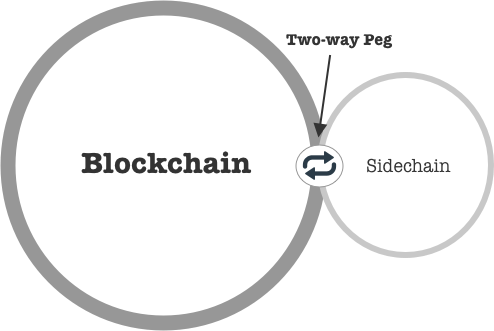
\includegraphics[scale=0.5]{../img/sidechain}
    \caption{Two-way pegged sidechain}
    \label{img:sidechain}
\end{figure}

Thanks to the possibility of using its own less decentralized but more scalable 
consensus algorithms, sidechains can provide a much higher throughput than a 
primary blockchain. However the introduction of consensus assumptions, which in 
situations of failure, will permanently compromise long-term guarantees such as 
persistence of asset ownership). If the state is “moved” to a sidechain and that 
chain’s consensus mechanism fails, owners or beneficiaries of that state may lose 
everything delegated to the sidechain, even in the case where the primary 
blockchain remains secure.

A slightly different approach can be taken with interoperable multi-chain networks 
such as \textit{Polkadot} (see figure \ref{img:polkadot}). Polkadot allows new 
designs of blockchains (also known as parachains) to communicate and pool their 
security while still allowing for entirely arbitrary state-transition functions. 
This helps with bootstrapping new chains much faster while having the same security 
guarantees as the whole of Polkadot network.

Slightly different approach is taken by interoperable multi-chain networks such 
as \textit{Polkadot} (see figure \ref{img:polkadot}) which allows new designs of
blockchains (called parachains) to communicate and pool their security while 
still allowing them to have the entirely arbitrary state-transition functions. 
This helps to bootstrap new chain much faster while having same security 
guaranties as whole Polkadot network.

\begin{figure}[H]
    \centering
    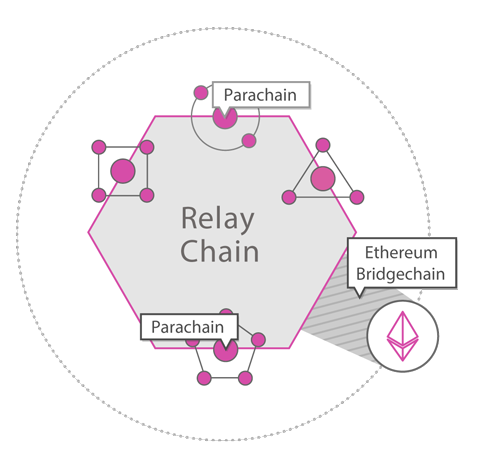
\includegraphics[scale=0.5]{../img/polkadot}
    \caption{Polkadot network components}
    \label{img:polkadot}
\end{figure}

\textit{Sidechains} can provide significant increase of transaction throughput, 
and in the case of multi-chains - relatively easily achievable high level of 
security guarantees. Despite this, general issues of blockchains still apply.

Blockchains by nature have physical networking and storage limitations. They are
still unable to provide throughput of hundreds of thousands of transactions per 
second and \textit{instant finality} - both fundamental requirements for 
micropayments in a successful decentralized VPN or streaming platform.

\subsection{Plasma}

\textit{Plasma} \cite{plasma} is a proposed framework for scaling Ethereum 
capacity by using hierarchical sidechains. Plasma type sidechains (also called
child chains) allow a majority of transactions outside of the “root chain” (e.g. 
Ethereum). Only deposits and withdrawals, and the points of entry and exit are 
handled by the root chain smart contract. 

Similarly to blockchains, Plasma chain stores all its transactions packed into 
blocks while using \textit{UTXO} for balance accounting. To make sure that 
transactions are final, Plasma operators run a “state commitment”. This is a 
cryptographic way to store a compressed version of the state of a child-chain 
inside of the root chain. Typically all states are stored in \textit{merkle trees}
and only the \textit{merkle root} of each block’s state is added to the root 
chain.

Although Plasma chains are run by single operators, having distributed nodes 
using some kind of Byzantine Fault Tolerant (BFT) consensus (e.g. Proof of Stake) 
is possible.

One of Plasma’s key differentiators is that it creates the possibility for users 
to leave the network at any time. This action is usually referred to as “exiting”. 
This allows users to safely withdraw their funds from Plasma even if it has been 
shut down by the operator.

While it offers significant speed (up to 1000 tx/s) and latency improvements over 
Ethereum itself, Plasma cannot offer the near-zero latency and near-free transaction 
fees required for a decentralized VPN micropayments solution. Plasma also requires 
significant storage to manage it’s ledger (especially with the large amount of 
transactions). \\

Plasma chain is that it is a complex and difficult to implement solution. What is 
especially hard with its implementation is that you are required to run distributed 
nodes which have BFT type of consensus. When Plasma chain is operated by a single 
operator, there is a risk that this operator will create “fake” blocks, which may 
result in mass exits out of Plasma into the root chain, affecting the entire 
network.

Another downside of Plasma chains is that it is quite expensive to operate. Every 
couple of blocks, it would have to commit its state to the root chain. This means 
that a plasma operator would have to pay \$1080 USD (gas fee) per day.

\[ 3 \thinspace tx / minute * 1 440 \thinspace minutes / day = 4320 \thinspace tx/day \]
\[ 1 \thinspace tx = 25 \thinspace cents \]
\[ 4320 \thinspace tx/day * 0.25 USD/tx = 1080 \thinspace USD/day \]

This isn’t such a big problem when there is a significant load on the network, 
however, in the beginning covering such costs can be problematic.

And finally, even though Plasma’s transaction throughput is significantly higher 
than Ethereum’s, it is still not enough for a decentralized VPN network’s needs. 
We could build some type of payment channels on top of Plasma (see figure
\ref{img:plasma-channels}). In this architecture, parties are able to do 
peer-to-peer transactions while having active service, and close channels right 
after ending the connection.

\begin{figure}[H]
    \centering
    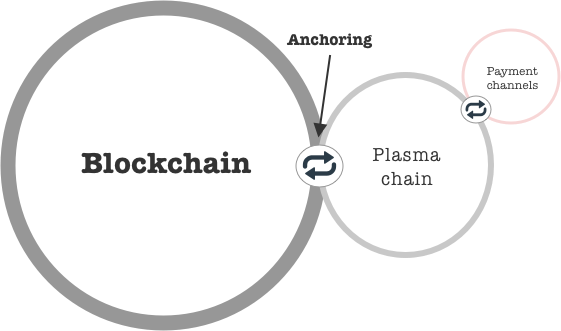
\includegraphics[scale=0.5]{../img/plasma-channels}
    \caption{Plasma + payment channels}
    \label{img:plasma-channels}
\end{figure}

In a situation when there is more than one transaction per second throughput, 
Plasma transactions can be relatively cheap (less than 1 cent per transaction) and 
can be quickly included into a block (from 1 to 10 seconds depending on the 
implementation). This allows consumers and providers in the network to open and 
close channels as and when needed, avoiding waiting times. 

Unfortunately this solution is even more complicated than using just Plasma and as 
such inherits similar cost and decentralization issues mentioned above.

\subsection{Payment and state channels based solutions}

A \textit{micropayment channel} is class of techniques designed to allow parties
to exchange digital value without commiting all of the transactions to the 
blockchain. With payment channels, an unlimited or nearly unlimited number of 
payments can be made between participants - with only the opening and closing of 
the channels being logged on blockchain. 

\begin{figure}[H]
    \centering
    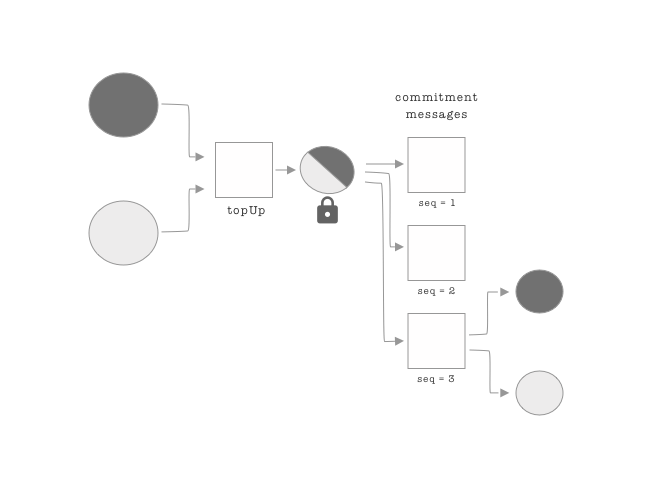
\includegraphics[scale=0.5]{../img/payment-channel}
    \caption{Sequense based payment channel}
    \label{img:payment-channel}
\end{figure}

To open payment channels both parties have to lock some funds into a multisig 
smart contract (see figure \ref{img:payment-channel}). This allows both parties
to update channel balances without the fear that funds will be double spent or 
stolen (to a high probability). 

There are various payment channel techniques - sequence based channels, duplex 
channels, time-locked channels, and more. Any of these would improve security and 
reduce the probability of double spending problems when compared to the initially 
proposed digital cheques solution (see section 2.2). This will also increase trust 
in the system, allowing providers to keep payment channels running for longer, 
reducing their settling costs.

\subsubsection{State channels}

State channels are the general form of \textit{payment channels}, applying the
same idea to any kind of state-altering operation normally performed on a 
blockchain. Moving these interactions off of the chain without requiring any 
additional trust can lead to significant improvements in cost and speed. State 
channels will be a critical part of scaling blockchain technologies to support 
higher levels of use.

The basic components of a state channel are very similar to payment channels.
\begin{enumerate}
    \item First, part of the blockchain state is locked via a multi-signature 
    smart contract. A specific set of participants must agree with each other 
    for updates within this smart contract.
    \item As they transact, participants update the state amongst themselves 
    by constructing and signing transactions. These states are held by both 
    participants, with each new update “trumping” the previous update.
    \item When all participants wish to settle, they can submit the state back
    to the blockchain, which closes the state channel and unlocks the smart 
    contract (usually in a different configuration than it started with).
\end{enumerate}

Because tokens on Ethereum blockchain are represented in the form of state in 
smart contracts, state channels are one of the through which token interactions 
can be moved into \textit{layer 2}. 

\subsubsection{Downsides and benefits of channels}

The downside of using payment channels is that both parties are required to lock 
funds into a multisignature smart contracts.\\

\textbf{\large {Disadvantages of State Channels}}
\begin{itemize}
    \item \textbf{Unnecessary transaction fees.} An additional on-chain transaction
    for opening the channel.
    \item \textbf{Locked in funds.} The need to have larger amounts of funds locked
    in the smart contract the inability to use funds locked in one channel before 
    closing the previous.
    \item \textbf{Time to service.} Opening a channel takes time. Depending on the 
    type of blockchain and network load, this may take from one minute to a couple 
    of hours.
    \item \textbf{Bad user experience.} Complexity in additional transactions and 
    long service time add up to an unfriendly and frictioned user journey.
\end{itemize}

\textbf{\large {Advantages of State Channels}}
\begin{itemize}
    \item \textbf{Privacy.} Each transaction is known only to participating 
    parties, allowing privacy in individual transactions. Only what is shared 
    on-chain will be publicly available.
    \item \textbf{Instant finality.} Parties can sign and exchange messages 
    instantaneously without having to wait for confirmation from the blockchain. 
    This will immensely improve user experience.
    \item \textbf{Lower cost.} Digital value is exchanged with the only a few
    on-chain transactions being made for creating and closing the channel.
\end{itemize}

\subsubsection{Micropayments networks}

Payments channels are a very promising technique for micropayments. However opening 
a new channel requires on-chain transaction. As mentioned, these are slow, expensive 
and aren't useful in networks with multiple service providers. In these cases, 
payment channel based solutions are reasonable only when participants do not need to 
be connected to everyone else (see figure \ref{img:many-to-many}).

\begin{figure}[H]
    \centering
    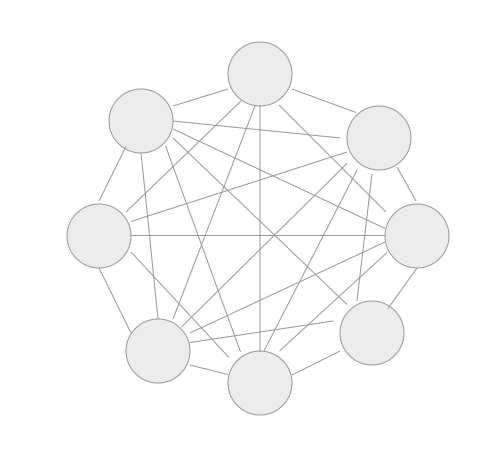
\includegraphics[scale=0.5]{../img/many-to-many}
    \caption{Everyone creates a channel with anyone else}
    \label{img:many-to-many}
\end{figure}

Existing research on payment channels have focused on exploring the design space of 
how to best structure payments through intermediaries \cite{counterfactual, perun, 
lightning}. Let’s suppose that Alice has a payment channel with Ingrid, and Ingrid 
has one with Bob. If Alice pays Ingrid off-chain and then Ingrid pays Bob the same 
amount, this equates to Alcie paying Bob off-chain, without requiring a new 
Alice-Bob payment channel.

In situation when parties do not have channels with a single intermediary, a 
micropayment channel network can be used together with a routing algorithm to send 
funds between any two parties in the network (see figure \ref{img:lightning}).

\begin{figure}[H]
    \centering
    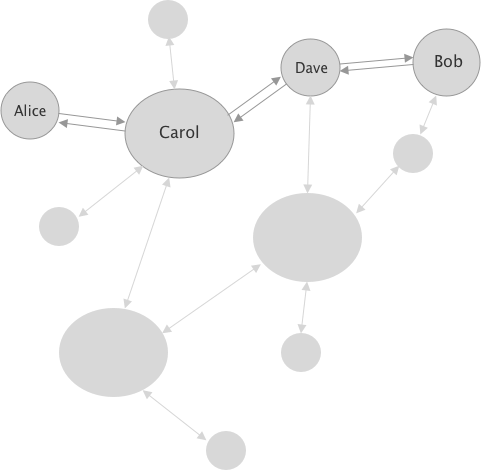
\includegraphics[scale=0.5]{../img/lightning-network}
    \caption{Micropayment channels network}
    \label{img:lightning}
\end{figure}

As micropayment channel networks can keep most transactions off-chain, blockchain 
based currencies may scale to magnitudes with larger volumes of users and 
transactions than currently existing centralized solutions. Also, micropayment 
channel networks allow for fast transactions thanks to their instant finality 
property. Transactions are final as soon as signed and sent to another party, and 
aren’t dependant on blockchain latency.

\subsubsection{Hashed Timelocked Contracts and Virtual Channels}

There are various ways to create micropayment networks trustlessly (i.e. to ensure 
that Alice pays Ingrid, if Ingrid pays Bob). The most popular of these methods are 
Hash Timelock Contract (HTLC) based approaches \cite{lightning}. Equal amount of 
funds from both payment channels are locked up in a way that only be released if 
a certain hash is revealed before a specific deadline. Thus canonically, locked 
“by hash” and “by time”.

This technique can allow payments to be securely routed across multiple payment 
channels. It is currently used in Bitcoin’s Lightning Network and Ethereum’s Raiden 
Network.

\begin{figure}[H]
    \centering
    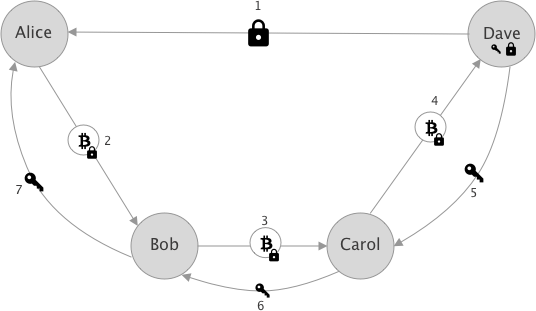
\includegraphics[scale=0.5]{../img/htlc}
    \caption{HTLC based payment - Alice pays Dave}
    \label{img:htlc}
\end{figure}

In figure \ref{img:htlc} we see atomic value exchange over three micropayment 
channels (Alice to Bob, Bob to Carol, Carol to Dave).\\

\textit{Step One:}
If Alice pays Dave via Bob and Carol, she needs to ensure that Bob and Carol cannot
run away with her money. To help ensure this, Dave generates pre-image $R$, which is 
a random number (shown as a key in the scheme), and shares hash $H$ of the pre-image 
(shown as lock on scheme) with Alice. 

\textit{Step Two:}
Alice generates an HTLC with Bob that says \textit{“I will pay you $X$ coins if you 
show me the pre-image $R$. If you don’t show $R$ during period $\Delta t$, I will 
take back my coins.”}

\textit{Step Three:}
Bob creates a similar HTLC with Carol, but sets the period of $\Delta t - 1$.

\textit{Step Four:}
Carol does same with Dave but with an even shorter period of $\Delta t - 2$.

\textit{Step Five:}
Dave shows $R$ to Carol.

\textit{Step Six:}
Carol shows $R$ to Bob.

\textit{Step Seven:}
Bob shows $R$ to Alice.

At this point payment of $X$ amount from Alice to Dave is finalised. 

HTLCs can be established in any chain of any length, consisting of different 
payment channels. As an incentive for intermediate hops to forward transactions,
small fees can be charged for using the service of the channel. Fee payments are 
also justified as the balance of a channel gets shifted, which is beneficial for 
balancing a lopsided channel. After successful transactions with HTLCs, channel 
parties do not need to broadcast their contract, and can just replace their HTLC 
with a new commitment transaction without an HTLC. HTLCs can be combined with 
timelocks or revocable transactions changing the output of the HTLC accordingly.\\ 

In the Ethereum blockchain, which supports advanced smart contracts, routing 
payments could be done using \textit{Virtual channels}, introduced by \textit{Perun}
paper \cite{perun}. A similar technique is proposed by Counterfactual protocol 
(named Meta channels) \cite{counterfactual}. These routing payments use an 
intermediary that serves as a \textit{“virtual payments hub”}. Anyone with a 
payment channel connected to the hub could establish virtual channels between each
other (see figure \ref{img:hub}). Unlike routing payments via HTLCs, Hub does not 
need to be involved in every payment between Alice and Bob. This property reduces 
latency and costs, while increasing privacy.

\begin{figure}[H]
    \centering
    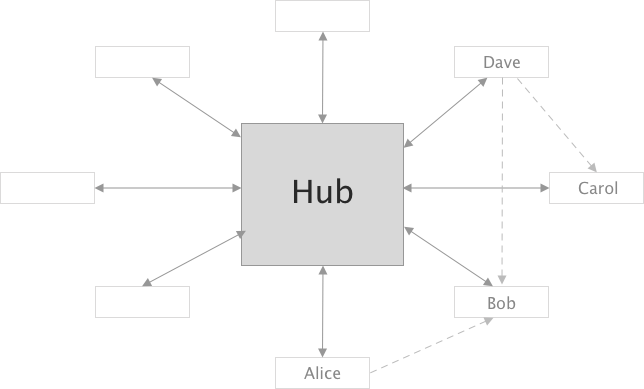
\includegraphics[scale=0.5]{../img/hub}
    \caption{Virtual Payment Channel Hub}
    \label{img:hub}
\end{figure}

To open a virtual channel, Alice and Bob essentially need to lock-up a set number 
of coins from their payment channel with Hub. The amount of locked coins will 
become the value of the virtual channel between Alice and Bob. Notice that the hub 
remains financially neutral, simply mirroring balances.

This technique could be reapplied to increase the length of the channel (see figure 
\ref{img:virtual-channels}). Because a virtual channel is an instance of an 
off-chain contract, increasing the length does not require an additional transaction
on-chain. 

\begin{figure}[H]
    \centering
    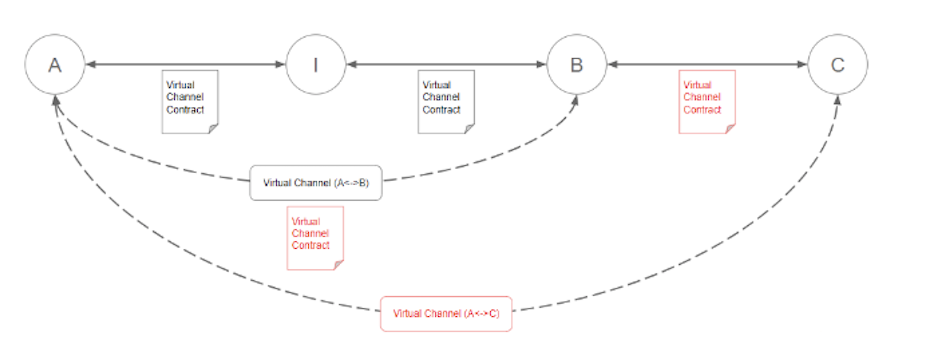
\includegraphics[scale=0.6]{../img/virtual-channels}
    \caption{Bob becomes the Hub for channel between Alice and Carol}
    \label{img:virtual-channels}
\end{figure}

Virtual channels also represent a different business model from channel routing. 
HTLCs have a nels also represent a different business model from channel routing.
HTLCs have a \textit{“pay-per-payment”} fee model where this is need to incentivize 
intermediaries to route payments. Virtual channels on the other hand have a 
\textit{“rent-a-path”} fee model. In this model an intermediary acts as a virtual 
payment hub that has direct channels with multiple parties.

If Ingrid is the intermediary, then Alice and Bob pay Ingrid to keep the channel 
open for a certain period of time. This model has potential to have better economics 
for high-volume micropayments. 

While Perun and Counterfactual have introduced novel means of routing payments 
across multiple intermediaries, HTLC-based routing is currently the primary 
implementation on blockchain mainnets making it the most tested. It is also easier 
to implement.

\subsubsection{Summary of problems within micropayment networks}

Micropayment channel networks look really promising, but unfortunately come with 
specific downsides. 

One of the first disadvantages of using HTLC based micropayment networks is the 
complicated routing that is required. \textit{Lightning Network} is great for time 
to time low value payments. However, it is much harder to use for frequent 
transactions to the same receiver due to the need to constantly check if all 
parties in the selected route are still alive and in useable conditions (i.e. each 
of the channels having enough funds to send payments forward). 

Complicated routing issues could be solved using the payment hub model, where one 
of a few intermediaries have a lot of channels with end users. The downside of this 
solution is that it requires the Hub to lock in a lot of funds in channels with all 
actors within the network. Another downside is that this solution is centralized. 
This means that if the hub’s operator is required to suspend activity or decides 
to shut down its servers, the whole network’s payment activities will come to a 
stop.

One of the critiques of payment channel networks is that both parties (paying and 
receiving) have to be on-line during payment. This issue is not valid for high 
frequence micropayments in decentralized networks due to the fact that both the 
provider and consumer have to be online for the service to be consumed.

Finally, micropayment channel networks are most useful with critical mass, and 
support in all popular programming languages and platforms. Unfortunately the most 
popular solution (Lightning Network) doesn’t support tokens. On Ethereum, there are 
a few promising projects (e.g. Raiden, Connext, Perun or Counterfactual), but they 
are in early stages of development and not widely adopted. This is partially due to 
the fact that they don’t come with rich tooling (e.g. protocol client 
implementations in popular languages like golang, rust or python). They are also 
quickly evolving pieces, that are changing rapidly, complicated to implement and 
hard to maintain. 

There are no clear winners at the moment. Trying to stick one of these into a 
general purpose payment network will mean a complicated migration into a more 
widely adopted solution in the future.

\subsection{Comparison and Conclusion}

They key insight of all \textit{Layer 2} solutions is that not every transaction 
has to be applied globally. All analyzed solutions solve this problem in different 
ways, with different trade-offs.

Many state channel developers see \textit{Layer 1} as the security layer and 
\textit{Layer 2} as the scalability layer. Furthermore, Layer 2 provides lower 
latency and cost per transaction, that is not possibly beyond a certain level 
of throughput within Layer 1 solutions.

\begin{table}[H]\footnotesize
    \centering
    \caption{Comparison of researched solutions}
    {\begin{tabular}{|l|c|c|c|c|c|} \hline
       & \textbf{Channels} & \textbf{HTLC Network} & \textbf{Payment Hub} & \textbf{Plasma} & \textbf{Sidechain} \\
      \hline
      On-chain transactions & $\bullet\bullet\bullet$ & $\bullet\bullet$ & $\bullet\bullet$ & $\bullet$ & $\bullet$ \\
      Instant finality &  \checkmark &  \checkmark &  \checkmark & & \\
      Hight throughput & $\bullet\bullet$ & $\bullet\bullet\bullet$  & $\bullet\bullet\bullet$ & $\bullet$ & $\bullet$ \\
      Off-chain messaging & $\bullet$ & $\bullet\bullet\bullet$ & $\bullet\bullet$ & $\bullet$ & $\bullet$ \\
      Decentralised & \checkmark & \checkmark & $\pm$ & $?$ & $\pm$ \\
      Requires specialised wallet & $?$ & \checkmark & \checkmark & \checkmark & \checkmark \\
      Topup from exchange & $?$ & $-$ & $-$ & $-$ & \checkmark \\
      Easily embeddable & \checkmark & $\pm$ & $-$ & $\pm$ & $\pm$ \\
      Overall user experience & $\bullet$ & $\bullet$ & $\bullet\bullet\bullet$ & $\bullet\bullet$ & $\bullet\bullet$ \\
      Implementation complexity & $\bullet$ & $\bullet\bullet\bullet$ & $\bullet\bullet$ & $\bullet\bullet\bullet$ & $\bullet\bullet\bullet$ \\
      Fast settlement & $?$ & $-$ & $\pm$ & \checkmark & $-$ \\
      Security & $\bullet\bullet\bullet$ & $\bullet\bullet\bullet$ & $\bullet\bullet\bullet$ & $\bullet\bullet\bullet$ & $?$ \\
      Utility token support & \checkmark & \checkmark & \checkmark & \checkmark & \checkmark \\
      \hline
    \end{tabular}}
    \label{tab:comparison}
\end{table}


\textbf{\large Glossary of Symbols:} \\
    $\bullet\bullet\bullet$ -- high, \\
    $\bullet\bullet$ -- medium, \\
    $\bullet$ -- low, \\
    \checkmark -- yes, \\
    $\pm$ -- more or less, \\
    $?$ -- unknown, depends on implementation. \\

\textbf{\large Glossary of terms:}
\begin{itemize}
    \item \textbf{Channels} -- pure payment channels bease solution (without 
    a network), when each pair of consumer and provider open a new communication
    path.
    \item \textbf{HTLC Network} -- Micropayment channels networks which uses hash
    timelocked contracts for payment routing (e.g. Raiden Network).
    \item \textbf{Payment Hub} -- Virtual channel hubs based payment solution, 
    such as Perun, Counterfactual or Connext.
    \item \textbf{Plasma} -- One of Plasma chain implementations (e.g. Plasma 
    MVP), dedicated to serve for payment purposes for particular distributed
    systems.
    \item \textbf{Sidechain} -- Running sidechains using Substrate or Tendermint
    frameworks and connected to Polkadot or Cosmos.
\end{itemize}

In table \ref{tab:comparison} we can see comparison of through analysis of the 
abovementioned solutions. It is clear that because of \textit{instant finality} 
and higher throughput possibilities micropayment channel based solutions (such as 
state channels, HTLC networks or virtual payment hubs) are better fits for high 
frequency micropayments on decentralized platforms.

\section{Accountant pattern - lightweight payment protocol}

After analyzing solutions in today’s market it is clear that at this stage it may 
be best to introduce our own lightweight, state channel based, easy to implement 
and maintain solution.

In this section we will articulate how the \textit{"Accountant pattern"} will be 
architected. Put simply, this solution will combine the best pieces of payment 
promises, unidirectional channels and payments using single intermediaries making 
use of hashed timelocked contracts so as to avoid the need for introducing trusted
custodians.

\subsection{Payments over "Accountant"}

Digital cheques or \textit{Payment promises} is elegant, efficient and easy to 
implement solution. They have to be signed by only one party, and are easily 
verifiable, simple to set up and unlimited in the amount of updates required to 
store only the last version of the issued promise.

The main disadvantage that these digital cheques or promise mechanism is that it 
introduces the possibility of double spending, which roll on to more regular 
on-chain settlements. To solve this problem, we propose introducing a new party 
into the network called the \textit{Accountant} which will have an overview of 
and verify promises issued by consumers. It would do this by being aware of the 
actual balance of each consumer’s funds (see figure 
\ref{img:unidirectional-payments}).

\begin{figure}[H]
    \centering
    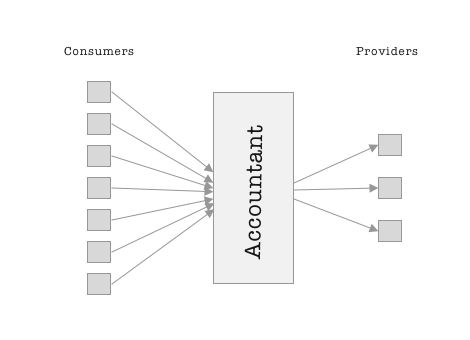
\includegraphics[scale=0.5]{../img/unidirectional-payments}
    \caption{Payments via Accountant}
    \label{img:unidirectional-payments}
\end{figure}

Accountant is the most complicated to implement part of this protocol. It has
to store the state of balance of each consumer and be able to accept many 
transaction valudation requests.

\begin{figure}[H]
    \centering
    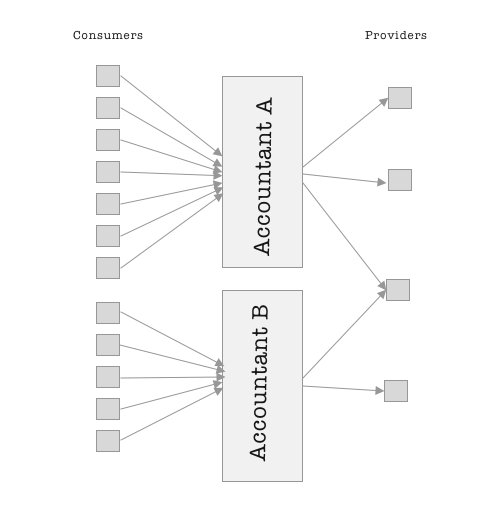
\includegraphics[scale=0.5]{../img/multi-accountants}
    \caption{Multiple accountants may be used in the network}
    \label{img:multi-accountants}
\end{figure}

To maintain the requirement of decentralization, there can be multiple accountants 
deployed in the network (see figure \ref{img:multi-accountants}). In the case of a 
decentralized VPN network, consumers will work with only one accountant, while 
providers will need to be aware of different accountants. 

Accountants are chosen by consumers, but because of cryptographic schemes described 
in the following sections, Accountant is non-custodial, can’t steal any funds or 
cooperate with consumer to cheat providers.

\subsection{Payment Promises based uni-directional channels}

To organise secure, non-custodian and trustless payments via Accountant, we have to 
maintain two types of channels: paying channels (consumer $\rightarrow$ accountant) 
and receiving channels (accountant $\rightarrow$ provider). As such, Accountant 
plays a similar role as an intermediary or hub described in section 3.3.3.

\begin{figure}[H]
    \centering
    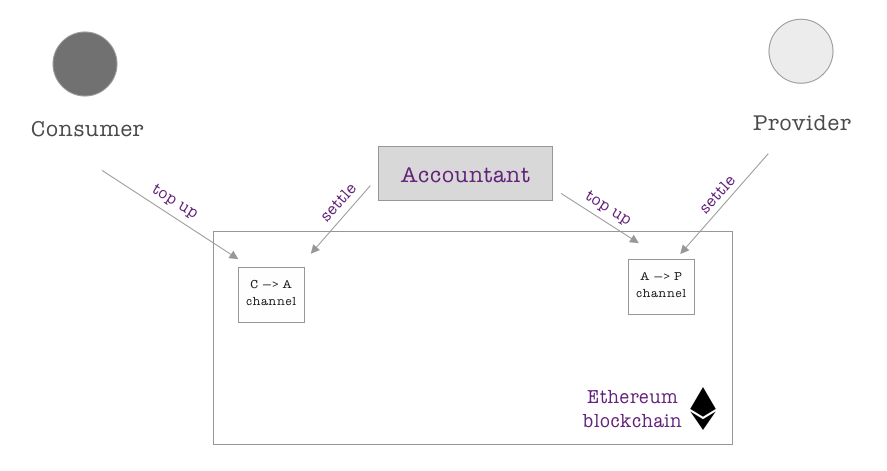
\includegraphics[scale=0.4]{../img/accountant-channels}
    \caption{Two types of channels}
    \label{img:accountant-channels}
\end{figure}

In the case of a decentralized VPN network, payments need to flow in one direction, 
from consumer to provider. We saw the potential in organising uni-directional state 
channels which are very similar to payment promises and have most of their 
properties. The key difference is the requirement of accounting and frozen funds 
for each channel. Also hashlock check (HTLC described in section 3.3.4) was added 
to guarantee that Accountant is unable to steal these funds.

Implementation of the promise settlement function can be found below, and the full 
state channel smart contract can be found in Mysterium Network’s GitHub repository 
\cite{smartcontracts}.

\begin{lstlisting}[language=Solidity]
    struct Party {
        address beneficiary; // funds destination
        uint256 settled;     // total amount already settled
    }

    function settlePromise(uint256 _amount, bytes32 _lock, bytes memory _signature) public {

        bytes32 _hashlock = keccak256(abi.encode(_lock));
        address _channelId = address(this);

        address _signer = keccak256(abi.encodePacked(
                _channelId, 
                _amount, 
                _hashlock
        )).recover(_signature);
        require(_signer == operator);

        // Calculate amount of tokens to be settled.
        uint256 _unpaidAmount = _amount.sub(party.settled);
        require(_unpaidAmount > 0);

        // If signer has less tokens than asked to transfer, 
        // we can transfer as much as he has already and rest 
        // tokens can be transferred via same promise but in 
        // another tx when signer will topup channel balance.
        uint _currentBalance = token.balanceOf(_channelId);
        if (_unpaidAmount > _currentBalance) {
            _unpaidAmount = _currentBalance;
        }

        // Increase already paid amount
        party.settled = party.settled.add(_unpaidAmount);

        // Send tokens
        token.transfer(party.beneficiary, _unpaidAmount);
    }
\end{lstlisting}

Since our channels are uni-directional instead of sequence number there is simply
used total promised amount. Smart contract are calculating difference between 
amount on given promise and already settled amount.

\[ amountToTransfer = totalPromised - alreadySettled \]

This provides a high level of flexibility. Promises can be settled in any order,
with any gaps. For example, only one of thousand payment promises can be send to 
settle and the amounts will still be calculated correctly.

\subsection{Identity registry}

Another important component of this protocol is a \textit{registry} where all 
identities - consumers, providers and accountants will be registered. Payment 
channels will be created between consumers and accountants during registration 
(see figure \ref{img:registration}). 

\begin{figure}[H]
    \centering
    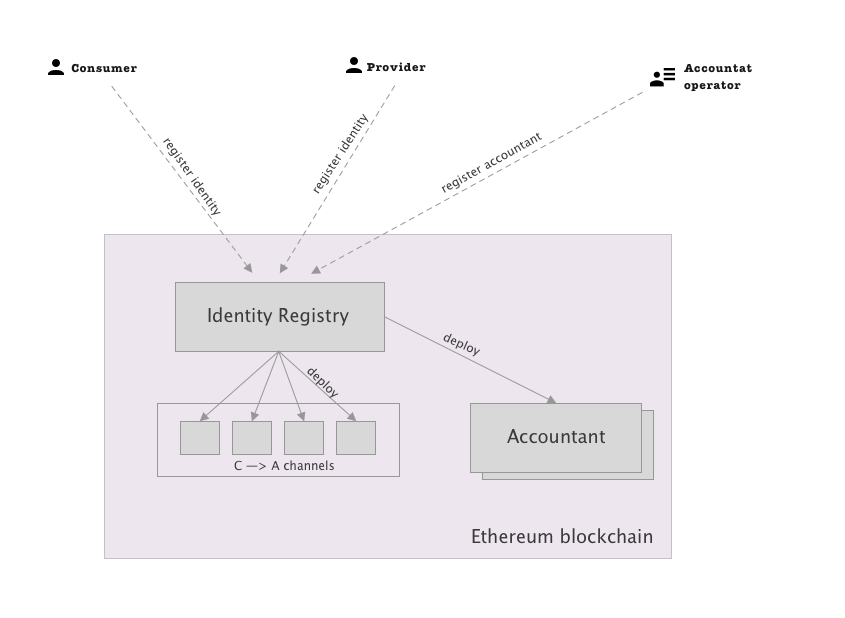
\includegraphics[scale=0.4]{../img/registration}
    \caption{Registration of Accountant and Identities}
    \label{img:registration}
\end{figure}

Since there will be no need to deploy a channel for each registered identity, 
there is an optimisation in terms of saving on channel deployment transaction 
fees. This protocol suggests the use of \textit{EIP1167} (Minimal Proxy Contract
\cite{eip1167}) which will proxy all requests into a single 
\textit{ChannelImplementation} contract while still allowing for the maintenance
of separate states and addresses per channel (see figure \ref{img:proxy}).

\begin{figure}[H]
    \centering
    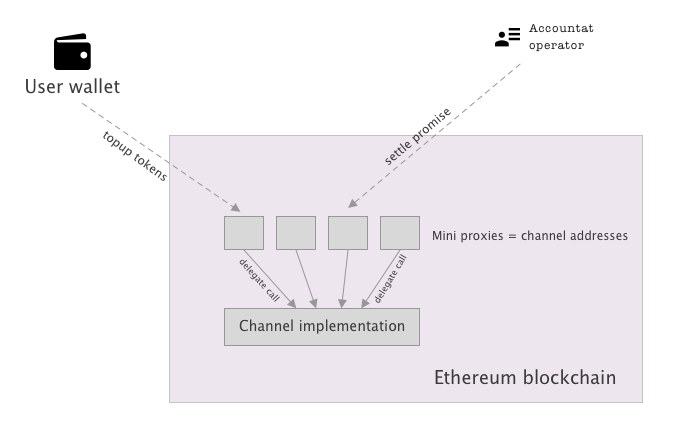
\includegraphics[scale=0.5]{../img/proxy}
    \caption{Minimal proxies pointing into a single implementation}
    \label{img:proxy}
\end{figure}

Consumer (paying) channels are deployed using \textit{CREATE2} opcode \cite{create2}
which allows deterministic calculation of the future channel address.

\[ keccak256(0xff + registry + identity + keccak256(byteCode))[12:]\]

This means that users can top up their channels even before registering an identity 
and an actual smart contract is deployed. Also due to the fact that each channel 
has a separate address, and it’s top up doesn’t require adding additional 
parameters (payload) to the transaction, these channels can be topped up using any 
wallet with token support, or directly from an exchange.

\subsection{Off-chain messaging and promise exchange}

The Accountant pattern differs from those in \textit{Lightning Network} or 
\textit{Hub} based payment networks in that these payments are not going through 
an intermediary, but are instead “verified” by Accountant. You can see the payment 
promise exchange technique in figure \ref{img:off-chain-interactions} below.

\begin{figure}[H]
    \centering
    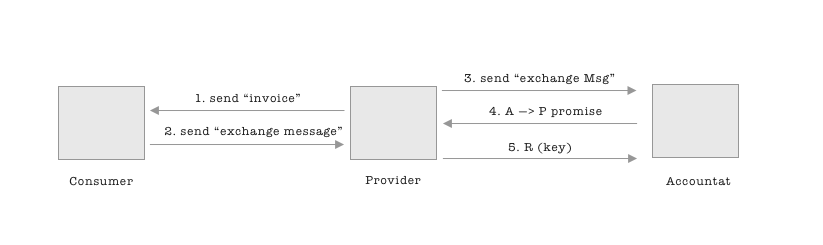
\includegraphics[scale=0.5]{../img/off-chain-interactions}
    \caption{HTLC based payment > Bob pays Alice}
    \label{img:off-chain-interactions}
\end{figure}

The payment is finalized in five steps. At first, the Provider will have to 
\textit{generate invoice} and send this to the Consumer.

\[ invoice = [hashlock, agreementId, agreementAmout] \]
\[ hashlock = keccak256(R) \]
\[ R = HugeRandomNumber \]

Then the Consumer issues payment promise, which allows the Accountant to settle 
given amount of funds, pack it into an \textit{Exchange message} and send it back 
to the Provider.

\[ Message = keccak256(channelId, totalPromisedAmount, hashlock) \]
\[ Signature = sign(Message) \]
\[ Promise = [Message, Signature]\]
\[ ExchangeMessage = [Promise, agreementId, agreementAmout] \]

In the next step, the Provider is exchanging promises with the Accountant. In the 
end the Accountant will have promises to settle funds in the Consumer’s channel and 
the Provider will have payment promises to settle the same amount of funds in the 
Accountant’s channel. 

\[ \Delta amount = newAgreementAmout - seenAgreementAmout \]
\[ totalPromisedAmount = previousPromisedAmount + \Delta amount \]

The provider can do the same promise exchange operations with many consumers at 
once. After any number of successful off-chain interactions, the Provider at any 
point in a single transaction can settle the accumulated value of payments by a 
couple of consumers (see figure  \ref{img:payment}). 

Additionally if the Provider is willing to take more risk, he can verify (exchange 
promises with the Accountant) in a lump sum, and reduce the amount of off-chain 
communication and fees paid to the Accountant.

\begin{figure}[H]
    \centering
    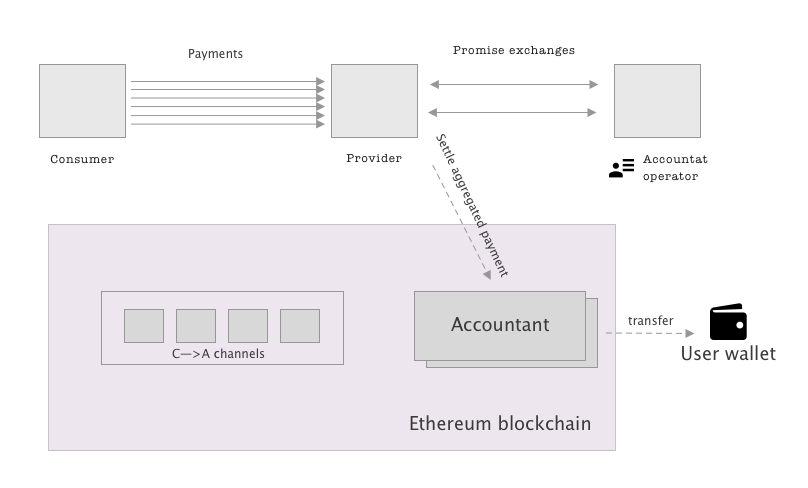
\includegraphics[scale=0.4]{../img/payment}
    \caption{Provider settles aggregated promise}
    \label{img:payment}
\end{figure}

Accountant is also accumulating payment promises given by the same Consumer to 
different Providers. When the Accountant has a payment promise with enough value, 
he can settle it on-chain (see figure \ref{img:accountant-rebalance}) and rebalance
paying and receiving channels.

\begin{figure}[H]
    \centering
    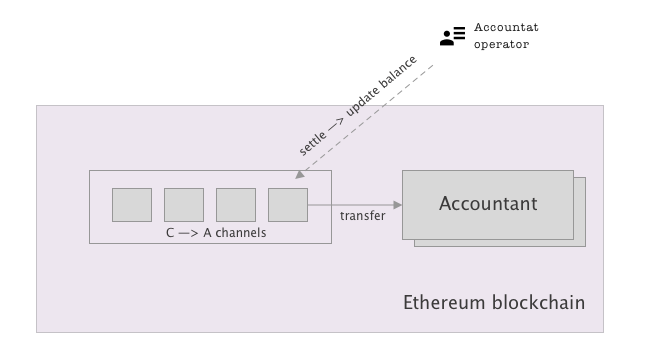
\includegraphics[scale=0.5]{../img/accountant-rebalance}
    \caption{Accountant rebalancing is simple settlement of collected promises}
    \label{img:accountant-rebalance}
\end{figure}

\subsection{Incoming channel funds guarantees, and trustless rebalance}

All analyzed micropayment channel based solutions have the common disadvantage of 
needing to lock funds in channels with each party. In hub based solutions, this 
problem is even bigger and requires a \textit{"rich hub"}. In a decentralized VPN 
network, it is possible to separate consumers are providers, and thereby decrease 
this problem.

\begin{lstlisting}[language=Vyper]
    lockedFunds: uint256 # amount of accountant funds already locked in channels
    struct Channel:
      loan: uint256      # amount lended by provider
      balance: uint256   # amount available to settle
      settled: uint256   # total amount settled by provider

    @public
    def rebalanceChannel(channelId: bytes32):
      newBalance: uint256 = channels[channelId].loan
      assert newBalance > channels[channelId].balance

      channel: Channel = channels[channelId]

      if(newBalance > channel.balance):
        lockedFunds += channel.balance - newBalance
        assert token.balanceOf(this) >= lockedFunds

      channel.balance = newBalance
\end{lstlisting}

Provider’s stakes can be taken and lent into the Accountant and immediately locked
in his receiving payment channel. This way the Accountant will lock his own funds, 
meaning that the Provider can settle payment promises in value of up to his stake 
size.

One of the additional benefits of this is that the Accountant can’t actually 
withdraw or use these funds, so channel rebalance can be  done by anyone, without 
the Accountant’s signature.

“Always online” is a big problem for payment channels. If the Provider is offline 
or is under DDoS attack, he will be unable to post the finalized state (during the 
dispute period) and the Accountant will have the possibility to take funds locked 
in the channel.

Our proposed method doesn’t run into this problem, because funds are double locked. 
The Accountant can’t leave the channel with more funds than his own locked part of 
balance. So if the Provider has an unsettled promise for a smaller amount than he 
lent to the Accountant, the Provider is safe and will be able to recover his funds, 
even if the Accountant “disappears” for a really long period of time.

\subsection{Transaction maker}

One of the most un-user friendly parts of transferring ERC20 tokens is the gas 
fees. This transfer operation takes a small fee in ethers to pay for gas. A second
problem that arises when working with smart contracts on Ethereum is that in order 
to call some function, a user would have to add a Payload (first 4 bytes of keccak 
of function’s signature). This introduces friction to the user journey and further, 
isn’t supported by many wallets or exchanges.

In the case of topups, this problem is solved thanks to the construct described in 
section 4.3. Unfortunately for identity registration and promise settlement, a 
user’s application (e.g. dVPN mobile app or provider’s node) would need to have ETH
topped up in there. This is inconvenient and creates problems both with onboarding 
advanced users, and educating beginners.

\begin{figure}[H]
    \centering
    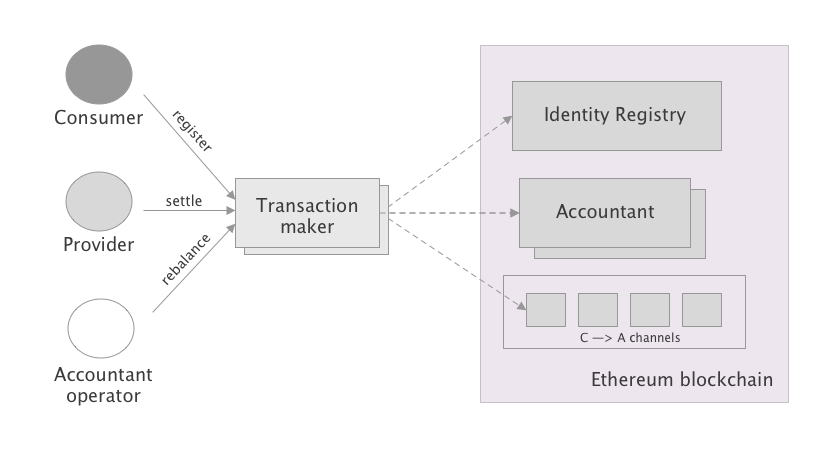
\includegraphics[scale=0.45]{../img/transactor}
    \caption{Communication with blockchain via Transaction maker}
    \label{img:transactor}
\end{figure}

For identity registration and promise settlements we may make use of an additional
service named \textit{"Transaction maker"}. The role of this service is to get 
user’s requests and send transactions into blockchain (see figure 
\ref{img:transactor}). 

All smart contracts created for the Accountant are constructed in a manner such 
that all their calls can be made from any account, simply by adding a channel 
operator signature as a parameter into payload. Additionally we construct payment 
promises in a way such that only one signature is needed and it is possible to 
settle them in any order with any gaps. This means that promises can be published 
publically without any risk of attack. 

There could be deployed as many such services as needed.vEach network participant 
could decide to use own \textit{"Transaction maker"}, or even there could be 
version of accountant operator software where such service is integral part.

Sending transactions into blockchain costs so users could cover that cost, but
instead of using additional currency (ethers in case of Ethereum), they could
pay in tokens.

There is potential misbehavior of \textit{"Transaction maker"}, when he is
getting paid but didn't do his job, or misbehavior of users when they decide
not pay after transaction was sent to blockchain by \textit{"Transaction 
maker"}. To resolve this problem, functions of smart contracts usually have fee
parameter in them.

\begin{lstlisting}[language=Solidity]
    function settlePromise(uint256 _amount, bytes32 _lock, uint256 _fee, bytes memory _signature) public {

        require(_amount >= _fee);
        
        ...

        // Send tokens
        token.transfer(
            party.beneficiary, 
            _unpaidAmount.sub(_fee)
        );

        // Pay fee for transaction maker
        if (_fee > 0) {
            token.transfer(msg.sender, _fee);
        }
    }
\end{lstlisting}

In this way \textit{"Transaction maker"} will get his reward only if he actually 
will send transtation and users have no chance to avoid fee.

\begin{figure}[H]
    \centering
    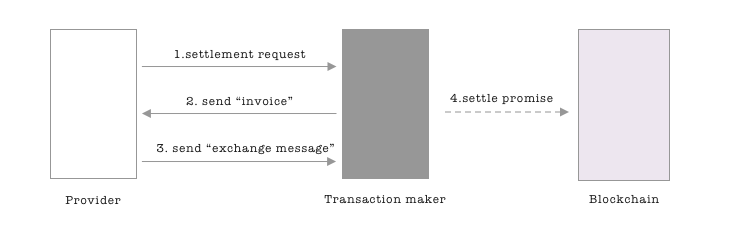
\includegraphics[scale=0.5]{../img/transactor-payment}
    \caption{Paying via Tramsaction maker flow}
    \label{img:transactor-payment}
\end{figure}

\subsection{Properties of the protocol}

This protocol was designed to be an integral part of certain decentralized systems. 
It has not been designed for general purpose payment network used in many 
applications and daily life where each parties can both receive and transfer funds.

Main properties of the protocol are:

\begin{itemize}
    \item Easy channel topup (even from an exchange).
    \item Payments aggregation $\Longrightarrow$ minimal on-chain transactions.
    \item Fast settlement into blockchain without the need for another party to 
    be online and cooperate.
    \item Guarantee of incoming channel balance/collateral size.
    \item Simple off-chain communication (one roundtrip payment).
    \item Possibility of avoiding the Accountant for at least part of the 
    transactions.
    \item Pull based interactions with Accountant $\Longrightarrow$ providers don’t
    have to be externally exposed or maintain live connection with the Accountant.
    \item Secure $\Longrightarrow$ double spend protection using non-custodian 
    accountant model.
    \item Fast channel opening $\Longrightarrow$ possibility not to wait until 
    opening tx will be mined.
    \item Instant finality of payments.
\end{itemize}

\section{Potential future work}

There are three main directions in which future development of payment solution
could evolve: 
\begin{itemize}
    \item migrate into Connext or Perun;
    \item migrate into Plasma + channels;
    \item add support of counterfactual channels for accountant pattern.
\end{itemize}

\subsection{Migration into Connext or Perun}

Two most closed and most promissing solutions to described Accontant pattern are
\textit{Perun virtual payment hubs} and \textit{Connext hub}. While Perun team 
is still working on their first version of protocol implementation, Connext team 
already working on thirs iteration of their hub solution (this time using 
Counterfactual state channels). Unfortunatelly at the moment both solutions are
not ready to use inside dVPN application written by Mysterium team. 

In Connext case, they're changing their solution a lot, so it's worth to wait 
until their implementation will stabilise. Also their client application is 
written in TypeScript which means that Mysterium would need to reimplement it 
in golang and take care of all protocol changes. Another problem is, that their
off-chain messaging is much more complicated and requires storing a quite a lot
of state by client nodes.

Perun team is creating their client node using golang, which makes it good
choice, but because protocol itself is complicated and implementation is in 
early stage, there is quite hard to say if it will work as expected and will
provide all needed features for good user experience (described in 2.3 section, 
7th requirement).

In the future, when these solutions will be more mature and if Accountat pattern
will not serve as expected, there may be made migration into one of these 
solutions.

\subsection{Plasma plus channels}

In Ethereum community there are a lot of development going aroud various Plasma 
implementations. Unfortunatelly each analysed Plasma implementation had own 
issues (either centralisation, either mass exit risk, either having support only
for non-fungible tokens). Additionaly, as was described in 3.2 section, in 
initial state running own Plasma could be expensive, and there are no popular
and decentralised Plasma implementation runned by thirs party teams.

In the future however, if there would be proposed Plasma implementation which
solves earlier mentioned problems, would have already developed tooling which
would help to run own implementaiton easily or they would appear decentralised
and popular solution implemented and runned by third party team, Mysterium team 
could easyly enough adapt their dVPN node software to use uni-directional, 
payment promise based channels on top of Plasma.

\subsection{Take use of Counterfactual state channels}

Generalized state channels described in Counterfactual \cite{counterfactual} 
white paper looks like very powerful sulution. Also we see that there is some
traction around this solution. If this trend will grow, in the future we may
take some effort to research possibility to refactor Accounant pattern proposed 
uni-directional channels and implement them in counterfactual way. Ideally there
could be possible to install them as an application on top of existing opened 
channel with counterfactual hub. This would help to have minimal changes inside 
dVPN node software but in same time be part of bigger network.

\newpage
\printbibliography[heading=bibintoc]

\end{document}
